\chapter{肌肉力量优化} \label{chap:chap9}

人类遇到的每一个问题总有一个众所周知的解决方案——简洁、合理,但又错误。
\begin{flushright}
	——H. L. 门肯
\end{flushright}


\begin{figure}[!htb]
	\centering
	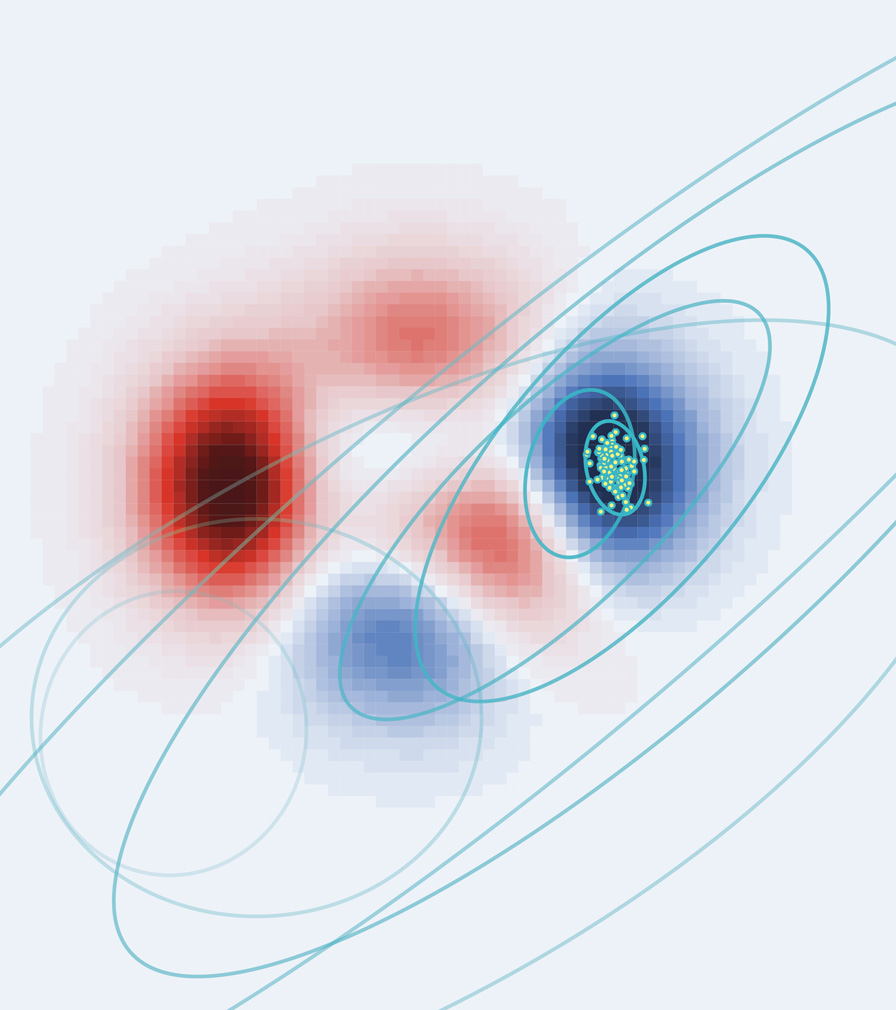
\includegraphics[width=1.0\linewidth]{chap9/9_0}
	% 加星号(*)表示不加编号
	\caption*{ \label{fig:9_0}}
\end{figure}


我一生中发现的最伟大的生物力学发现之一并非源于实验室,也未借助任何特殊设备,仅仅依靠人体不可思议的适应性。
1968年,一位名叫迪克$\cdot$福斯贝里的21岁土木工程系学生公布了他的发现,并在奥运会上以向后跳过跳高横杆的方式震惊了体育界。
一位体育记者写道:“福斯贝里跳过横杆就像一个人被人从30层楼的窗户推下去一样。”
然而,正是这种看似笨拙的跳高方式,让他创造了2.24米的奥运纪录,并最终获得金牌。


福斯贝里实际上是在高中时出于无奈才开始使用他的标志性技术。
他没能掌握当时的标准技术——“西部翻滚”,即跳高运动员面朝下越过横杆,仿佛用手臂和腿环抱横杆。
他还尝试了更古老的“剪刀”技术,即跳高运动员以近乎坐姿的姿势越过横杆,同时双腿像剪刀一样上下摆动。
但这种技术并不理想,因为跳高运动员必须将重心推到远高于横杆的高度。


在背越式跳高中,跳高运动员先向横杆一端跑去,然后向内弯曲身体,向中间跃过横杆,最后在最后一刻扭转身体,向后跃过横杆(图~\ref{fig:9_1})。
身体每次只滑过一个部位:
首先是头部和肩部,然后是躯干、臀部、膝盖,最后是双脚。
背越式跳高的一个优点是身体重心无需越过横杆。
在最高高度,臀部位于横杆上方时,背部拱起,头部和腿部悬在横杆下方,从而降低了重心。


\begin{figure}[!htb]
	\centering
	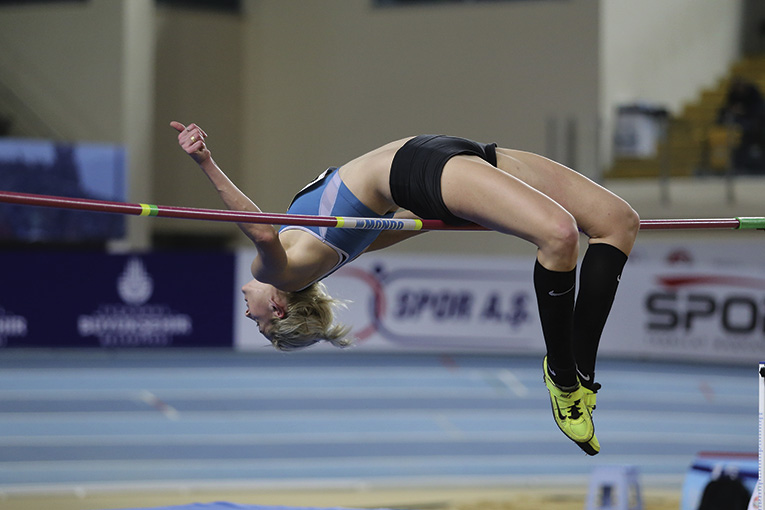
\includegraphics[width=1.0\linewidth]{chap9/9_1}
	\caption{“背越式跳高”跳高技术。
		玛雅扬$\cdot$弗曼-沙哈夫的照片,摄影:埃夫伦$\cdot$卡林巴卡克。 \label{fig:9_1}}
\end{figure}


尽管福斯贝里在发明背越式跳高时并未接受过任何正规的生物力学训练,但我们现在已经赶上了他开创性的天才。
如今,教练们使用高速录像来指导跳高运动员脚部着地的位置、蹬地前蹲到多低等等。
他们想到了福斯贝里从未想过的改进。
起跳时抬起手臂可以增加垂直动能。
臀部越过横杆后收下巴有助于迫使臀部下沉,并根据牛顿第三运动定律,将双脚抬起并越过横杆。


自1980年以来,所有跳高世界纪录都是用背越式跳高创造的,其他所有技术都已从世界舞台上消失。
现在争论的焦点是哪种背越式跳高最好:
“速度背越式”还是“力量背越式”?


对我来说,福斯贝里跳马的故事教会了我几个宝贵的教训。
首先,我们永远不应该想当然地认为流行的做事方式就是唯一或最佳方式。
但一个不那么哲学、更偏向生物力学的信息是,我们的身体拥有关节骨骼和数百块肌肉,赋予我们完成任务的无限可能,无论是像端咖啡这样看似简单的动作,还是像跳两米高这样复杂的动作。
每一个动作都需要我们的大脑协调肌肉活动。
下巴的一个简单的动作就能对我们的双脚产生影响。


为了完成任何动作,我们的身体都会解决一个优化问题,试图用最小的努力获得最大的效果。
但有一个问题,无论是数学模型还是现实世界的运动员,都可能遇到难题:局部最优并不总是全局最优。
在背越式跳高之前的运动员们都认为他们找到了最佳技术。他们错了。
但他们无法仅仅通过对西方的滚翻技术进行小幅(“局部”)调整来提高标准。
他们需要一位愿意进行大规模(“全局”)调整的运动员工程师,来改变我们对跳高应该是什么样子的理解。


在本章中,我们将探讨两种使用数值优化计算肌肉力量的广泛场景。
第一种场景出现在我们希望估算产生可观测运动的肌肉力量时。
由于人体肌肉骨骼系统存在冗余,因此通常存在许多可能的解,我们将应用优化方法,找到符合某些标准的最佳肌肉力量集。
我们将这个问题称为肌肉冗余问题(也称为肌肉力量共享问题)。
第二种场景出现在研究肌肉协调性以优化特定任务(例如跳高)的表现时。
在这种情况下,我们需要计算肌肉力量以及完成任务的身体节段运动。
如果为优化器提供跳高比赛规则和足够逼真的肌肉骨骼系统模型,它就能发现背越式跳高(以及其他我们可能从未见过的技术)。
需要注意的是,使用优化方法估算肌肉力量不仅仅是为了计算上的便利:神经系统本身就是一种优化器。
让我们来深入了解一下细节。


\section{生物和数值优化器}

人们有意识地优化他们的日常生活。
我们会决定如何分配时间、金钱、注意力和其他有限的资源,以最大限度地平衡短期和长期的满足感,并在遵守法律和其他义务等约束的同时做到这一点。
令人惊讶的是,人类也会在潜意识中优化。
回想一下第二章,我们会自然地调整步行速度、步频和其他步态变量,以使我们的交通成本接近最低——当然,除非我们赶时间,在这种情况下我们会优先考虑速度而不是代谢成本。
在学习新任务和适应新情况时,我们也会在优化过程中,根据具体情况最大化准确性、效率、舒适度和其他性能指标的某种组合。
实验表明,我们会维持一个关于身体的“内部模型”,即潜意识地理解我们刺激肌肉的程度与由此产生的身体部位运动之间的关系。
当我们置身于新环境,例如国际空间站的微重力环境或机器人装置施加的人工力场时,我们最初会显得笨拙且效率低下,因为我们在规划和预测自身动作时使用的是一个不再精准的内部模型。
在探索新环境的过程中,我们会利用视觉和其他感官反馈来调整内部模型,提高协调性。
随着时间的推移,我们会适应新环境,并通过重新学习肌肉兴奋与运动表现之间的关系,重新获得熟练的技能。


数值优化算法使用类似的探索性或“猜测-检验”策略来寻找欠定问题的解。
我们将这些猜测称为候选解,每个候选解都为所有未知数或设计变量(例如肌肉冗余问题中的肌肉激励)提供了一个数值。
每个候选解的适用性通过评估目标函数或成本函数来确定,成本函数是量化特定设计变量值集合的可取性的表达式。
能够提供最佳目标函数值(视情况而定,最小值或最大值)的候选解被称为最优解,或者简称为优化问题的解(请注意,我们可以将我们的任务定义为始终寻求最小化目标函数;为了最大化像跳跃高度这样的量,我们只需最小化其负值即可)。
正如我们将看到的,目标函数的选择会对解以及计算它所需的工作量产生深远的影响。


最优解也会受到约束条件的影响。
在许多问题中,我们要求候选解满足某些表达式(等式或不等式),才能使其成为可行解或可接受的解。
例如,在肌肉冗余问题中,我们要求所有肌肉力均为拉伸力,并且它们产生的力矩之和等于所需的净关节力矩(例如,使用逆动力学算法计算)。
由于约束条件只能减少可行解的数量(即减小解空间的大小),因此,受约束优化问题的解的目标函数值并不比优化问题不受约束时更好。
添加约束会减少您的选择。
如果约束条件过多,解空间可能为空(问题可能没有可行解)。
根据研究问题的不同,可以将一个或多个严格约束转换为软约束,这些软约束以“惩罚”的形式添加到目标函数中。
惩罚项通常通过加权因子进行缩放,以便根据其相对重要性调整它们对目标函数的贡献。
通用优化问题可以表述如下:
%
\begin{proposition}[优化问题 1:找到产生所需关节力矩的踝跖屈肌力量] \label{pro:optim_1}
	
	\begin{equation}
		\begin{matrix}
			\text{最小化} & $ J(\underline{x}) $  & \text{调整设计变量 $ \underline{x} $ 以最小化目标函数 $ J(\underline{x}) $} \\
			% 
			$\text{受约束}$ & g_i(\underline{x}) \leq 0, i=1,...,n^i  & \text{同时满足 $ n $ 个不等式约束,} \\
			%
			& h_j (\underline{x}) = 0, j=1,...,n^j  &  \text{满足 $ n $ 个等式约束,} \\
			& \underline{x}^\text{lower} \leq \underline{x} \leq \underline{x}^\text{upper} & \text{并尊重设计变量的界限。}
		\end{matrix} \nonumber
	\end{equation}
	
\end{proposition}


我们潜意识地运用同样的原理来协调肌肉。
想象一下拿起桌上一支笔的动作。
你知道手所需的最终位置和方向,但你可以自由地(在一定范围内)选择手臂的最终姿势以及达到该姿势的路径。
正式地说,这个问题的每个候选解可能提出一组不同的肌肉激励,这些激励被定义为时间的参数化函数;这些参数将成为设计变量。
在所有候选解中,可行解是那些描述实现所需最终手部姿势的肌肉激励模式的解。
其他约束条件可能描述其他不可协商的要求,例如避开障碍物。
你大概会寻求在一定程度上最小化行程时间,但目标函数也可能包含一个有利于减少肌肉力量的项,用于完成这项非紧急任务。
解决此类问题的一种简单方法是评估所有可行解的目标函数,然后选择最佳候选解。
然而,正如您所料,所谓的“穷举搜索”(即考虑所有可能性)对于除最简单问题之外的所有问题都是低效且不切实际的。
数值优化器会尝试通过评估其认为必要的候选解数量来找到最有利的可行解(或至少是足以解决当前问题的可行解)。
许多优化器的区别仅在于它们如何根据已探索的候选解的适用性来选择新的候选解进行评估。


现在,我们将转向讨论解决肌肉冗余问题的策略。
为简单起见,我们将在某一时刻寻求解,假设所需的净关节矩已知,且对象静止不动。
我们有时将此类问题称为“静态”优化问题,因为其中忽略了一些与时间相关的因素。
在下一节中,我们将构建一个优化问题陈述,并通过观察求解一个简单的肌肉冗余问题,以建立对解空间的直觉。
在接下来的章节中,我们将讨论一些能够解决现实世界中遇到的非平凡优化问题的数值算法。



\section{通过检查解决静态优化问题}

我们首先关注图~\ref{fig:9_2}~所示的模型。假设我们希望产生 100 N$ \cdot $m 的踝关节跖屈净力矩。
应该激励哪些肌肉来产生这个力矩呢?有很多可行的方案。
例如,也许整个期望力矩都应该由比目鱼肌产生,或者最好是模型中的三个跖屈肌各自贡献一部分力矩。
背屈肌也可以产生力量,也可以由其中一块或两块背屈肌产生。
因此,该问题是欠定的:方程的数量少于未知数,我们需要更多信息来解决这个问题。
正式表述为,我们希望找到由每块肌肉 $ i $(我们的设计变量)产生的力 $ F_i $,使得踝关节跖屈总力矩为 100 N$ \cdot $m(等式约束),但前提是 $ F_i $ 为正,且对于任意 $ i = 1, ..., 5 $(界限)。


\begin{figure}[!htb]
	\centering
	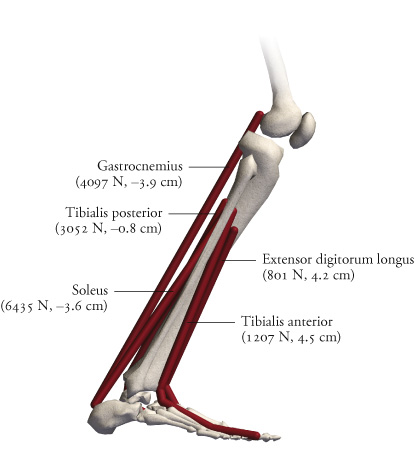
\includegraphics[width=0.75\linewidth]{chap9/9_2}
	\caption{小腿和足部的肌肉骨骼模型,包含关键的跖屈肌和背屈肌。
		测量的踝关节力矩可能由多种肌肉力量组合产生。
		括号中的值是瞬时最大力(假设速度为零且肌腱刚性)以及所示姿势对应的踝关节力臂。 \label{fig:9_2}}
\end{figure}


解决欠定问题的一种方法是修改问题,使方程的数量与未知数的数量相同。
在我们的示例中,为简单起见,我们假设背屈肌处于非活动状态,产生的力为零。
这一假设将未知数的数量从五个减少到三个:腓肠肌(我们称之为 $ F_\text{GAS} $)、比目鱼肌($ F_\text{SOL} $)和胫骨后肌($ F_\text{TP} $)产生的力。
然而,我们仍然只有一个方程(指定期望净踝关节力矩的等式约束)。
我们可以假设每块跖屈肌都会产生相同的力,并引入 2 个附加方程,$ F_\text{SOL} = F_\text{GAS} $ 和 $ F_\text{TP} = F\text{GAS} $。
这种策略可以得到一个可行的解,但通常不会产生生理上合理的结果。
相反,我们将定义一个目标函数 $ J(\underline{F}) $,它将解的有利性量化为肌肉力的函数,然后求解以下优化问题:
%
\begin{proposition}[优化问题 1:找到产生所需关节力矩的踝跖屈肌力量]

\begin{equation}
	\begin{aligned}
		\text{最小化} & J(\underline{F})  &  \text{目标函数中较小的值更受青睐} \\
		\text{受限于} & 0.039 F^\text{GAS} + 0.036 F^\text{SOL} + 0.008 F^\text{TP} & \text{肌肉必须产生所需的净踝关节力矩} \\
		& 0 \leq F^\text{GAS} \leq 4097 & \\
		& 0 \leq F^\text{SOL} \leq 6435 & \text{肌肉力量必须在生理范围内} \\
		& 0 \leq F^\text{TP} \leq 3052 &  \nonumber
	\end{aligned}
\end{equation}

\end{proposition}


例如,假设我们假设神经系统最小化每个时刻产生的总肌肉力,因此这就是瞬时肌肉力的总和:
%
\begin{equation}
	J ( \underline{F} ) = 
		\triangleq
		F ^\text{GAS} + 
		F ^\text{SOL} + 
		F ^\text{TP} 
		= \sum_{i=1}^{3} F_i
	\label{eq:9_1}
\end{equation}

本例中的解是 $F^\text{GAS} = 2564$、$F^\text{SOL} = 0$ 和 $F^\text{TP} = 0$,因为腓肠肌具有最大的力臂,因此可以用最小的力量产生所需的踝关节跖屈力矩。
需要注意的是,在本模型中,腓肠肌能够产生完整的 100 N$\cdot$m 跖屈力矩(即 2564 N < 4097 N),实际上,当腓肠肌完全激活时,它可以在此姿势下产生约 160 N$\cdot$m 的力矩。
超过 160 N$\cdot$m 的踝关节力矩可以通过募集比目鱼肌(力臂第二大的肌肉)来产生,然后在比目鱼肌也达到最大力量后,再募集胫骨后肌(图~\ref{fig:9_3})。

\begin{figure}[!htb]
	\centering
	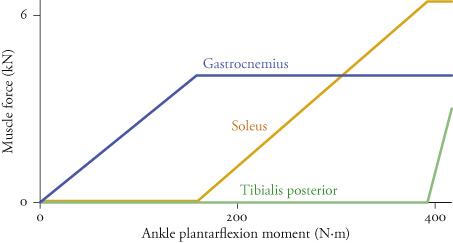
\includegraphics[width=0.75\linewidth]{chap9/9_3}
	\caption{图~\ref{fig:9_2}~中,假设肌肉协调策略最小化肌肉力量总和,则每块肌肉施加的力量会产生踝关节跖屈力矩。
		该目标函数(公式~\ref{eq:9_1})会导致不切实际的行为,即每块肌肉在下一块肌肉被调动之前就达到了其最大力量。 \label{fig:9_3}}
\end{figure}


虽然公式~\ref{eq:9_1}~中的目标函数可以很容易地求解优化问题,但请注意,当需要 100 N$\cdot$m 的跖屈力矩时,只会募集一块肌肉。
如果需要更大的力矩,则只有当第一块肌肉达到其最大产力能力时,我们才会募集第二块肌肉。
我们从实验中得知,肌肉实际上并非以这种逐步、非合作的方式募集。


不同的目标函数会导致不同的解决方案。
生物力学文献中提出了一些更切合实际的目标函数,但这些目标函数会导致无法通过检验解决的优化问题。
通常,我们必须使用计算机来解决生物力学中遇到的非线性、约束、高维问题。
在接下来的部分中,我们将讨论两大类优化算法:局部方法和全局方法。
然后,我们将继续解决一个更切合实际的肌肉力共享问题。



\section{解决静态优化问题的局部方法}

局部优化方法从一个初始猜测(候选解)开始,生成一系列新的猜测,每个猜测都与其前一个猜测相邻,并且通常具有更优的目标函数值。
当算法达到局部最优值时终止:该解在其紧邻域中被劣质解包围。
局部方法的一个典型示例是最速下降算法。
例如,如果我们求解一个二元最小化问题,目标函数 $J(x,y)$ 可以表示为一个曲面,其在点 $(x^*,y^*)$ 处高于 X-Y 平面的高度为 $J(x^*,y^*)$。
最速下降策略可以想象为将一颗弹珠放在目标函数曲面上,让它滚下山坡,直到落到盆底。
如图~\ref{fig:9_4}~所示,最终解取决于初始猜测,并且可能不是最佳解。
牛顿法与最速下降法类似,但它利用目标函数曲面的二阶导数(曲率)信息,更直接地逼近局部最小值——尽管计算这些额外信息的成本可能相当高。
内点法也很流行,它首先找到任意可行解(即可行域内部的解),然后在可行域内逐步寻找更优解。


\begin{figure}[!htb]
	\centering
	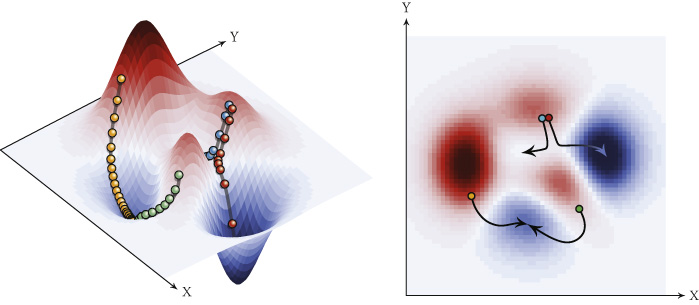
\includegraphics[width=1.0\linewidth]{chap9/9_4}
	\caption{两个变量目标函数的图形表示,其中曲面高度表示目标函数值 $J(x,y)$。
		最速下降算法从解空间中的某个点开始,沿着局部斜率最大的方向逐步下行,直到沿任何方向移动都能使 $J(x,y)$ 增加。
		最终解取决于初始猜测值,如此处所示的四条路径所示,并且可能并非全局最优。 \label{fig:9_4}}
\end{figure}


在图~\ref{fig:9_5}~中,我们展示了优化问题~\ref{pro:optim_1}(上文)的解决方案,该方案针对所有可能的踝关节跖屈力矩,同时最小化肌肉激活平方和,该平方和已被用作代谢能量消耗的替代品:


\begin{figure}[!htb]
	\centering
	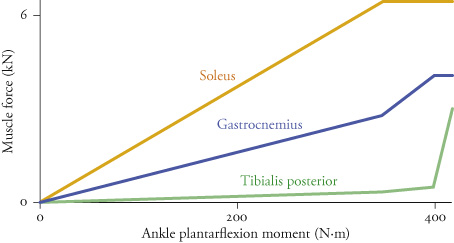
\includegraphics[width=1.0\linewidth]{chap9/9_5}
	\caption{图~\ref{fig:9_2}~中,假设肌肉协调策略最小化肌肉激活平方和,则每块肌肉为产生所有可能的踝关节跖屈力矩而施加的力。
		(公式~\ref{eq:9_2})得出的行为与实验观察结果一致,即即使产生微小的关节力矩,也会调动多块肌肉。 \label{fig:9_5}}
\end{figure}

\begin{equation}
	J ( \underline{F} ) 
		\triangleq 
		\sum_{i=1}^{3}
			( \frac{F_i}{F_i^\text{max}} )^2
		= 
		\sum_{i=1}^{3} a_i^2
	\label{eq:9_2}
\end{equation}


使用公式~\ref{eq:9_2}~计算出的肌肉活动比使用公式~\ref{eq:9_1}~所示的更简单的目标函数更接近人体实验中观察到的情况。
特别需要注意的是,在图~\ref{fig:9_5}~中,即使只需要较小的踝关节跖屈力矩,所有 3 块肌肉都会被募集,这与肌电图 (EMG) 的实验测量结果(图 9.6)在定性上相似。


\begin{figure}[!htb]
	\centering
	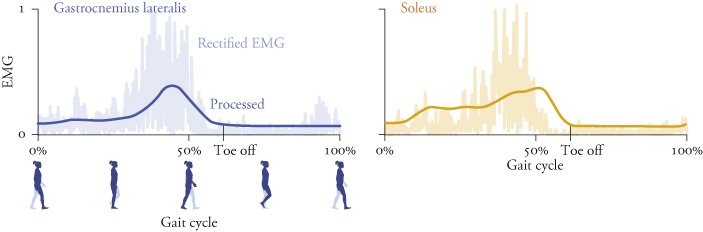
\includegraphics[width=1.0\linewidth]{chap9/9_6}
	\caption{行走时腓肠肌外侧肌(左)和比目鱼肌(右)的肌电图 (EMG) 信号。
		这两块肌肉都参与踝关节跖屈力矩的产生。数据来自 Bartlett 和 Kram (2008);Arnold 等人 (2013)。 \label{fig:9_6}}
\end{figure}


局部方法寻求其邻域内的最优解;然而,这样的局部最小值可能有很多。
例如,如图~\ref{fig:9_4}~所示,梯度下降算法找到的解取决于初始猜测。
我们或许可以尝试用不同的初始猜测运行该算法几次,但这仍然可能错过更好的——甚至可能好得多的——解。
记住迪克$\cdot$福斯贝里(Dick Fosbury)的名言。
因此,尽管局部方法可能很快,但全局方法可能会产生更好的解。



















